\documentclass[conference]{IEEEtran}
\IEEEoverridecommandlockouts
% The preceding line is only needed to identify funding in the first footnote. If that is unneeded, please comment it out.
\usepackage{cite}
\usepackage{microtype}
\raggedbottom
\emergencystretch=3em
\usepackage{amsmath}
\usepackage{amsmath,amssymb,amsfonts}
\usepackage{algorithmic}
\usepackage{tikz}
\usetikzlibrary{shapes, arrows, positioning}
\usepackage{array}
\usepackage{graphicx}
\usepackage[hidelinks]{hyperref}
\usepackage{textcomp}
\usepackage{xcolor}

\def\BibTeX{{\rm B\kern-.05em{\sc i\kern-.025em b}\kern-.08em
    T\kern-.1667em\lower.7ex\hbox{E}\kern-.125emX}}
    
\begin{document}

\title{ ASIC Implementation of Optimized Low Power High Speed ALU Using Booth Multiplier and Barrel Shifter  \\

}
\author{\IEEEauthorblockN{Nandini Mohangekar}
\IEEEauthorblockA{\textit{Dept.of Electronics and Communication} \\
\textit{KLE Technological University}\\
Belagavi, India \\
nandinimohangekar@gmail.com}
\and
\IEEEauthorblockN{Aditya Dhaded}
\IEEEauthorblockA{\textit{Dept.of Electronics and Communication } \\
\textit{KLE Technological University}\\
Belagavi, India \\
adityadhaded9@gmail.com}
\and
\IEEEauthorblockN{Akshaya Goudar}
\IEEEauthorblockA{\textit{Dept.of Electronics and Communication} \\
\textit{KLE Technological University}\\
Belagavi, India \\
akshayavgoudar555@gmail.com}
\and
\IEEEauthorblockN{Deepak Kajagar}
\IEEEauthorblockA{\textit{Dept.of Electronics and Communication} \\
\textit{KLE Technological University}\\
Belagavi, India \\
deepakkajagar2005@gmail.com}
\and

\IEEEauthorblockN{Ashwini Desai}
\IEEEauthorblockA{\textit{Dept.of Electronics and Communication} \\
\textit{KLE Technological University}\\
Belagavi, India \\
ashwinidesai.mss@kletech.ac.in}

\and
\IEEEauthorblockN{Sushant Jadhav}
\IEEEauthorblockA{\textit{Dept.of Electronics and Communication} \\
\textit{KLE Technological University}\\
Belagavi, India \\
sushantjadhav.mss@kletech.ac.in}
\and
}
\maketitle

\begin{abstract}
Arithmetic Logic Units (ALUs) are fundamental components of modern processors, embedded systems, and ASIC(Application Specific Integrated Circuit) based computing platforms, where speed, power efficiency, and hardware utilization significantly influence overall system performance. Typical ALU designs result in higher delay and hardware complexity, especially for shift and multiply operations. In this paper, design and ASIC implementation of an optimized 32-bit low power and high speed ALU, which combines Booth Multiplier and Barrel Shifter architectures are presented. To enhance the use of the opcodes and to decrease the complexity of the opcode decoder, the proposed design presents a common opcode mechanism with a 3-bit selection signal and an extra control signal, op\_switch. The entire architecture is designed in Verilog HDL and tested using Cadence NCLaunch and Xcelium and Cadence SimVision tools based on the conventional Front-End VLSI design flow. Functional verification confirms the successful execution of all eight supported operations. The proposed architecture realizes a multiplication delay of 2.42 ns and a shift delay of 0.66 ns, with about 87\% reduction in shift energy than the conventional architecture. Results from the simulations show better hardware utilization, lower complexity of control, more efficient operations and reliable operation for all the operations supported. The proposed ALU architecture is a good solution for ASIC applications which require low power consumption or high speed, such as embedded processors, digital signal processing systems, FPGA accelerators, and modern VLSI computing platforms.
\end{abstract}

\begin{IEEEkeywords}

ALU, Booth Multiplier, Barrel Shifter, ASIC, Verilog HDL, Cadence SimVision, VLSI

\end{IEEEkeywords}

\section{Introduction}

Arithmetic Logic Units (ALUs) are among the most important components of modern processors and embedded systems, as they execute arithmetic, logical, multiplication, and shift operations required during instruction processing. Since the ALU forms a major part of the processor datapath, its performance directly influences the speed, power consumption, and overall efficiency of the computing system. With the growing adoption of embedded systems, Internet of Things (IoT) devices, digital signal processing (DSP), and portable electronics, the demand for ALUs that provide higher performance with lower power consumption has increased considerably.

To address these challenges, several researchers have proposed improved ALU architectures by optimizing arithmetic units, multiplier designs, and shifting mechanisms.~\cite{ref1} presented a 32-bit ALU using optimized adder architectures to improve speed and reduce power consumption. ~\cite{ref2} incorporated a 32-bit Barrel Shifter to enable efficient single-cycle shift operations, while ~\cite{ref3} developed a low-power Barrel Shifter using transmission gate technology. Yeh ~\cite{ref4} proposed a high-speed Booth encoded multiplier that minimizes the number of partial products, thereby improving multiplication efficiency. In addition,~\cite{ref5},~\cite{ref6}, and ~\cite{ref7} demonstrated that optimized ALU and multiplier architectures can achieve better computational performance with reduced hardware complexity.

Despite these advancements, many existing designs focus on optimizing either multiplication or shift operations independently. Integrating both functionalities within a single ALU while maintaining low area, reduced power consumption, and simple control logic remains a challenging design objective.

This work presents a 32-bit ALU that integrates a Booth Multiplier and a Barrel Shifter within a unified architecture. The design is implemented using Verilog HDL and verified through Cadence simulation and synthesis tools. A shared opcode mechanism, based on a 3-bit selection signal and an additional \texttt{op\_switch} control signal, enables multiplication and shift operations to share the same opcode, reducing decoder complexity and improving hardware resource utilization. Experimental results demonstrate that the proposed ALU performs arithmetic, logical, multiplication, and shift operations efficiently, making it suitable for embedded processors, DSP applications, ASICs, FPGA-based systems, and other modern VLSI applications.

\section{Literature Survey}


Arithmetic Logic Units (ALUs) play a significant role in modern processors and digital systems by performing arithmetic and logical operations efficiently. Several researchers have proposed different techniques to improve ALU performance in terms of speed, power consumption and hardware complexity. Phanindrakumar et al. proposed a low-power and high-performance 32-bit ALU using different full adder architectures in 45nm CMOS technology \cite{ref1}. Their work focused on reducing propagation delay and power consumption using Hybrid CMOS logic techniques. Various full adder designs were analyzed using Cadence tools, and the proposed architecture demonstrated improved speed and reduced power dissipation compared to conventional ALU implementations.Rakshith et al. presented a Verilog HDL based implementation of a low-power and high-speed 32-bit Arithmetic and Logic Unit integrated with a barrel shifter architecture \cite{ref2}. The proposed design supports arithmetic, logical and shift operations while achieving reduced delay through single-cycle shifting. Similarly, Vudatha et al. proposed a low-power barrel shifter using Transmission Gate technology in 90nm CMOS technology \cite{ref3}. Their work focused on minimizing power dissipation and propagation delay during shifting operations, demonstrating the effectiveness of optimized barrel shifter architectures in VLSI systems.Multiplication is another critical operation affecting ALU performance. Yeh et al. proposed a high-speed Booth encoded parallel multiplier architecture using Modified Booth Encoding (MBE) techniques \cite{ref4}. Their approach reduced the number of partial products generated during multiplication, resulting in lower delay and improved computational efficiency. The study highlighted the importance of optimized multiplier architectures in achieving high-speed arithmetic operations.From the literature survey, it is observed that most existing ALU architectures focus on improving arithmetic performance, reducing power consumption and enhancing shift and multiplication operations through optimized hardware structures. However, limited attention has been given to optimizing ALU control logic and opcode utilization. The proposed work addresses this limitation by implementing a low-power and high-speed 32-bit ALU with optimized control logic, Barrel Shifter and Booth Multiplier architecture, thereby improving hardware utilization and reducing overall design complexity.
\section{Proposed System Architecture}
The proposed ALU architecture consists of four major modules:

\begin{itemize}
\item ALU Core
\item Booth Multiplier
\item Barrel Shifter
\item Shared Opcode Control Logic
\end{itemize}

Two 32-bit operands A and B are fed to the ALU; the operations are controlled by the signal sel[2:0]. Both operations, shift and multiplication, use the same opcode, with the op\_switch control signal.

The architecture simplifies the complexity of the control logic and enhances the efficiency of using the opcodes.

\subsection{Input Parameters}

\begin{itemize}
\item A[31:0] : First 32-bit operand
\item B[31:0] : Second 32-bit operand
\item sel[2:0] : Operation selection signal
\item op\_switch : Selects SHIFT or MULTIPLY operation
\item shamt[4:0] : Shift amount
\item shift\_mode[1:0] : Shift mode selection
\end{itemize}

\subsection{Output Parameters}

\begin{itemize}
\item Y[31:0] : ALU output result
\item carry : Carry flag
\item overflow : Overflow flag
\item zero : Zero flag
\item negative : Negative flag
\end{itemize}

\section{Operation Selection}

\begin{table}[h]
\centering

\renewcommand{\arraystretch}{1.3}
\setlength{\tabcolsep}{6pt}

\caption{Operation Selection Table}

\begin{tabular}{|c|c|c|}
\hline
\label{tab:opcode}
\textbf{sel[2:0]} & \textbf{op\_switch} & \textbf{Operation} \\
\hline
000 & X & ADD \\
\hline
001 & X & SUB \\
\hline
010 & X & AND \\
\hline
011 & X & OR \\
\hline
100 & X & XOR \\
\hline
101 & 0 & SHIFT \\
\hline
101 & 1 & MULTIPLY \\
\hline
110 & X & NOT \\
\hline

\end{tabular}

\end{table}

\subsection{Operation Selection and Opcode Mapping}
The proposed ALU has 3-bit selection signals \texttt{sel[2:0]} and an extra control signal \texttt{op\_switch} to select the ALU operation. The proposed design uses a shared opcode scheme to allow one opcode to be used for all operations, making the decoder circuitry and hardware less complex. The opcodes for both the SHIFT and MULTIPLY operations are the same (\texttt{101}), and the op\_switch signal controls which operation is used. If \texttt{op\_switch=0} the Barrel Shifter output is selected, and if \texttt{op\_switch=1} the Booth Multiplier output is selected. The ALU core performs arithmetic and logical operations (ADD, SUB, AND, OR, XOR, and NOT). Using combinational control logic and multiplexers, the operation selection is implemented and is used to route the output of the proper functional unit. The common opcode design minimizes decoder hardware, increases hardware efficiency, decreases power consumption and facilitates future ASIC and VLSI applications of the ALU. The operation mapping is shown in Table~\ref{tab:opcode}.

\section{Functional Flow Diagram}

\begin{figure}[h]
\centering
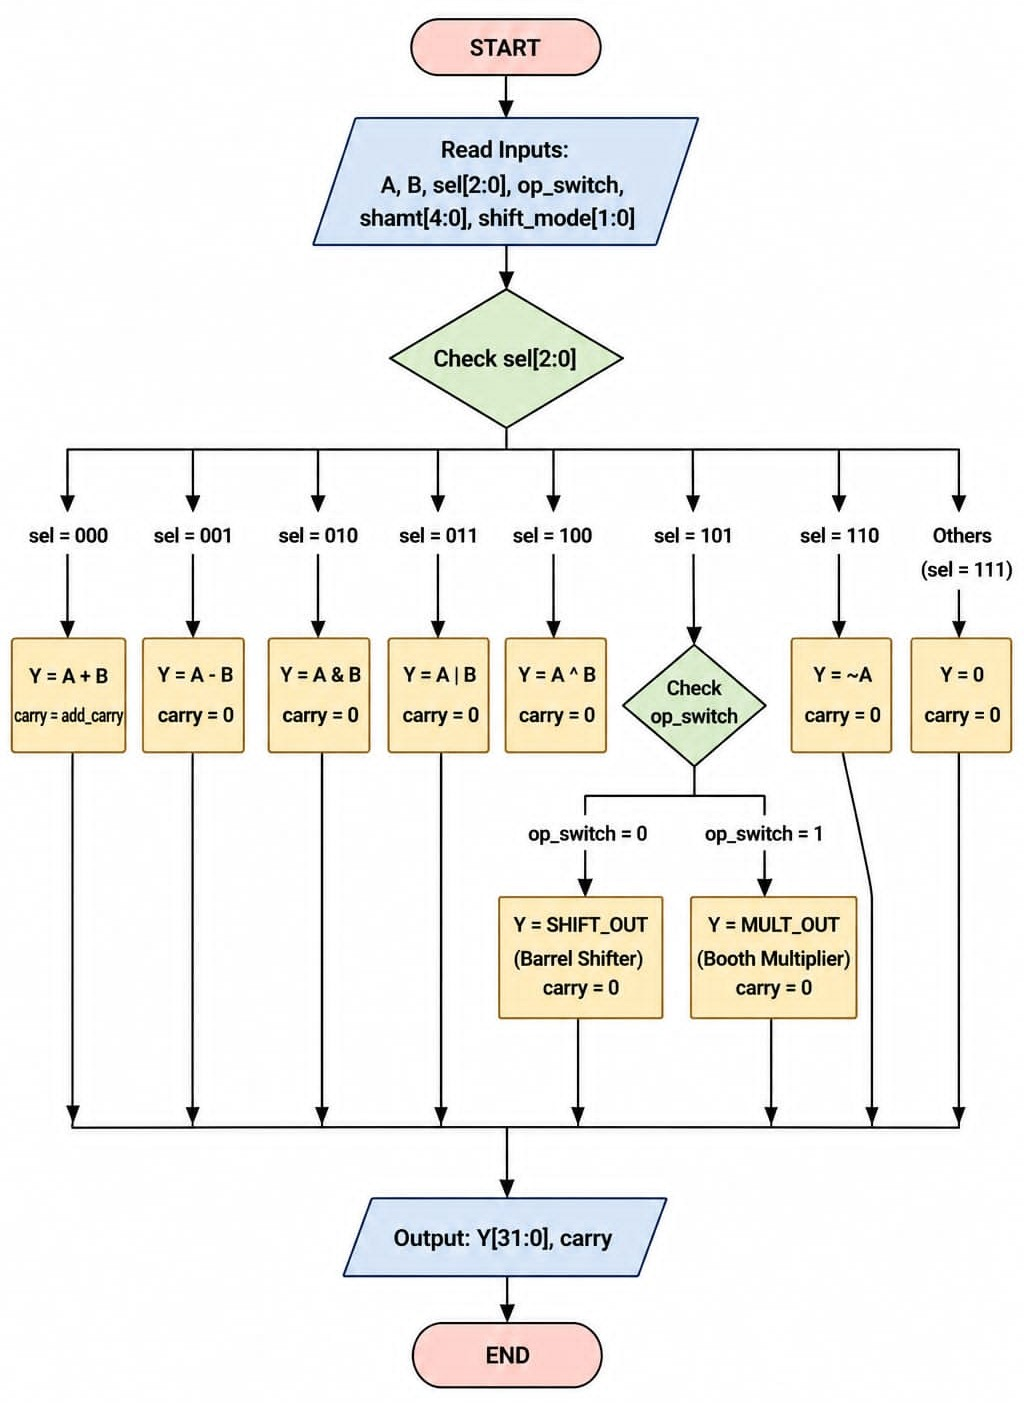
\includegraphics[width=8cm]{flowdiagram.png}
\caption{Functional Flow Diagram}
\label{fig:flow}
\end{figure}

Fig.~\ref{fig:flow} illustrates the functional flow of the proposed ALU architecture.
The operands to be used by the proposed ALU are input operands \(\texttt{A}\), \(\texttt{B}\), \(\texttt{sel[2:0]}\), \(\texttt{op\_switch[1:0]}\), \(\texttt{shamt[4:0]}\), and \(\texttt{shift\_mode[1:0]}\). The selection signal is a 3-bit value that is decomposed into activating the appropriate functional unit. The ALU Core performs arithmetic and logical operations like ADD, SUB, AND, OR, XOR and NOT. If the shared opcode (\texttt{101}) is chosen, then the operation is determined by a signal called the \texttt{op\_switch} signal. When \texttt{op\_switch=0}, the Barrel Shifter performs Logical Shift Left (LSL), Logical Shift Right (LSR) or Arithmetic Shift Right (ASR) operations, based on the shift amount and shift mode signals. The Booth Multiplier performs the multiplication of two operands \(A\) and \(B\) if \texttt{op\_switch=1}. The outputs of the ALU Core, Barrel Shifter and Booth Multiplier are multiplexed together to choose the final result for the ALU according to the value of \texttt{sel[2:0]} and the value of \texttt{op\_switch}. This functional flow is ideal for decoder logic, efficient hardware use, and for high speed, low power operation for ASIC and VLSI applications.

\section{Booth Multiplier Design}
\begin{figure}[h]
\centering
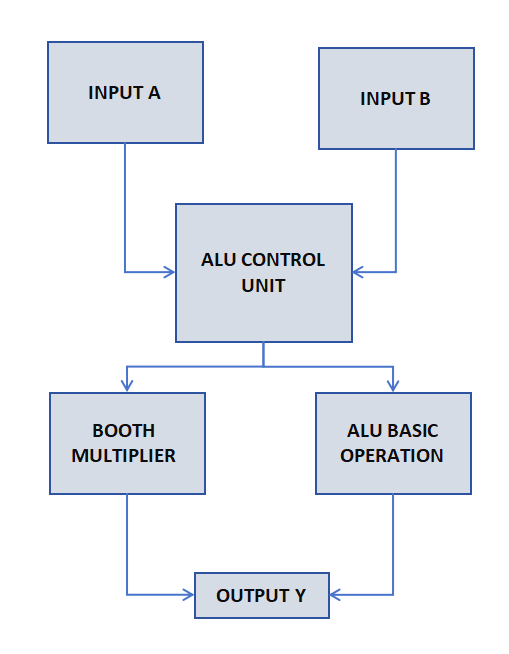
\includegraphics[width=0.30\textwidth]{booth_multiplier1.png}
\caption{Booth Multiplier Functional Block Diagram}
\label{fig:booth}
\end{figure}
Multiplication is the most expensive operation in the ALU. The conventional multiplication approaches create a huge number of partial products, which causes high hardware complexity, propagation delay and power dissipation. Hence the development of an efficient multiplier architecture is crucial for designing high speed and low power ALUs.The proposed ALU uses a Booth Multiplier to enhance the multiplication efficiency. The reason why Booth multiplication is widely used in digital systems is that it employs adjacent bits of the multiplier to minimise the number of partial products. This reduces the number of additions and subtractions operations, hence accelerates the computation, reduces hardware requirements and power consumption and is appropriate for VLSI and ASIC applications.The simplified behavioral modeling approach is used in this work for the implementation of the multiplier. The multiplication operation is described by a direct Verilog assignment, instead of using the complete Booth encoding algorithm with multiple iterative stages:

\begin{equation}
Y = A \times B
\end{equation}

Cadence Genus, a modern synthesis tool, automatically identifies the multiplication operator and performs an optimized synthesis of the hardware implementation internally. This saves the RTL designer from designing the appropriate multiplier architecture, and lets the synthesis tool do it for the designer.A and B are two 32-bit operands and the Booth Multiplier returns the multiplication result. The proposed ALU will use the lower 32 bits of the product as an output. When shared opcode is selected and op\_switch signal is logic 'high', the multiplier is activated.The integration of the Booth Multiplier in the proposed ALU structure is shown in Fig.~\ref{fig:booth}. The ALU Control Unit takes in the operands and control signals, and if the control signal is multiplication, the Booth Multiplier will generate the product and the ALU output will be connected to the product by the operation selection logic.The Booth Multiplier has been implemented in conjunction with shared opcode control and Barrel Shifter, improving the arithmetic performance but with minimal hardware complexity, so the proposed ALU is suitable for modern VLSI systems based on ASICs.
\section{Barrel Shifter Design}
\begin{figure}[h]
\centering
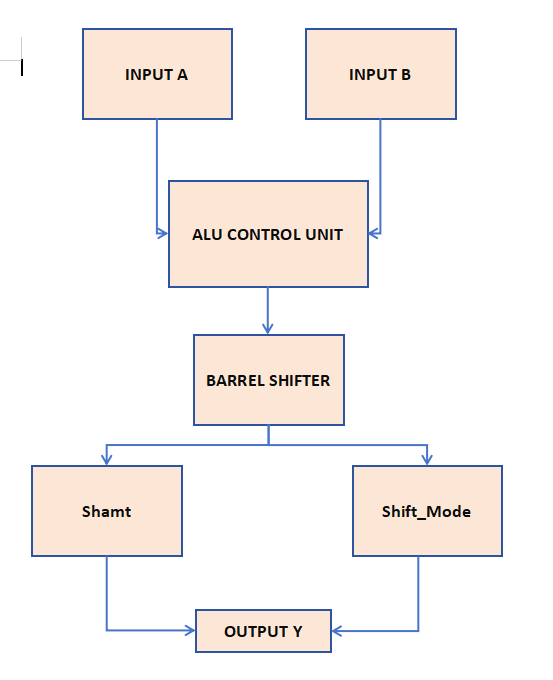
\includegraphics[width=0.30\textwidth]{barrel_shifter1.png}
\caption{Barrel Shifter Functional Block Diagram}
\label{fig:barrel}
\end{figure}
The functional organization of the Barrel Shifter integrated in the proposed ALU is shown in Fig.~\ref{fig:barrel}. The ALU Control Unit sends the shift amount (\texttt{shamt}) and shift mode signals to the Barrel Shifter, which is responsible for shifting the data in the ALU by a number of bits according to the shift mode signal. The shift operation is commonly used in digital processors for performing multiplication, division, address computation, alignment and bit manipulation. Unlike the conventional sequential shifter which takes several clock cycles to shift data by a number of bits equal to the shift count, the proposed Barrel Shifter is a combinational circuit that can shift data by any number of positions in just a single clock cycle. It takes a 32-bit operand and a 5-bit shift amount, allowing shifts of up to 31 positions and increasing the speed of shift execution and the reduction in shift latency.

The Barrel Shifter proposed is implemented in a parallel multiplexer based architecture with 5 stages corresponding to the shift value of 1, 2, 4, 8, and 16 bits. There is a shift operation at each stage, which transfers the input by one bit depending on the control signals, so that any shift can be performed in one operation. In the Verilog HDL implementation, \texttt{<<}, \texttt{>>} and \texttt{>>>} is used to implement the LSL, LSR and ASR operations respectively. This behavioral modeling approach makes RTL design easier and the synthesis tools can automatically produce optimized hardware. The ALU proposed in this work differs from the traditional ALU in terms of faster shift operations, lesser complexity in hardware, lower power consumption and superior performance, which makes it suitable for modern ASIC and VLSI applications.


\section{Implementation and Verification Environment}

The designed Arithmetic Logic Unit (ALU) is a 32-bit ALU, which has been designed based on the standard Front-End VLSI design process. The entire architecture has been described in Verilog Hardware Description Language (HDL) and functionally verified by Cadence simulation's. The design is divided into several modules: the ALU Core, Barrel Shifter, Booth Multiplier and a top level integration module. A testbench was built to test the correctness of all the supported operations.At first, the RTL design was implemented in Verilog HDL with the modular design approach. The individual modules were implemented and integrated to create the full ALU architecture. The design provides to support the arithmetic, logical, multiplication and shifting operations with a common opcode control.
The simulation has been conducted at functional level using cadence NCLaunch/Xcelium environment to confirm the responses of the design. Several test vectors were used in the testbench to verify the arithmetic, logic, shift, multiplication and operation selection logic. Cadence SimVision was used for analysis of the generated waveforms to verify proper operation of the entire system.The proposed design was developed on a Linux workstation, running Red Hat Enterprise Linux 8.7. The computing environment for the workstation was the Intel Core i5 processor, 7.4 GB RAM, and 64-bit operating system. This platform was used for simulation and verification of the ALU architecture.
The Front End VLSI design flow adopted in this work is summarized below:

\begin{enumerate}
\item RTL design with Verilog HDL.
\item Functional simulation using Cadence NCLaunch/Xcelium,
Verification with a testbench,Waveform Analysis using Cadence SimVision.
\item Designing and preparing for ASIC implementation in Cadence Genus,Generating netlist for further physical design using Cadence Innovus.
\end{enumerate}

The following are the implementation environment and tools for the project:

\begin{itemize}
\item Verilog HDL
\item Cadence NCLaunch/Xcelium
\item Cadence SimVision
\item Cadence Genus
\item Cadence Innovus
\end{itemize}

The implementation platform consisted of Red Hat Enterprise Linux 8.7 running on an Intel Core i5 processor with 7.4 GB RAM and a 64-bit operating system. The design targets a 180 nm CMOS technology platform.

The simulation and verification results showed that all the supported ALU operations were successfully executed. The reliable functionality and suitability of the proposed architecture for low power and high speed ASIC applications were achieved through the modular implementation approach together with the Front-End VLSI flow.

\begin{figure}[h]
\centering
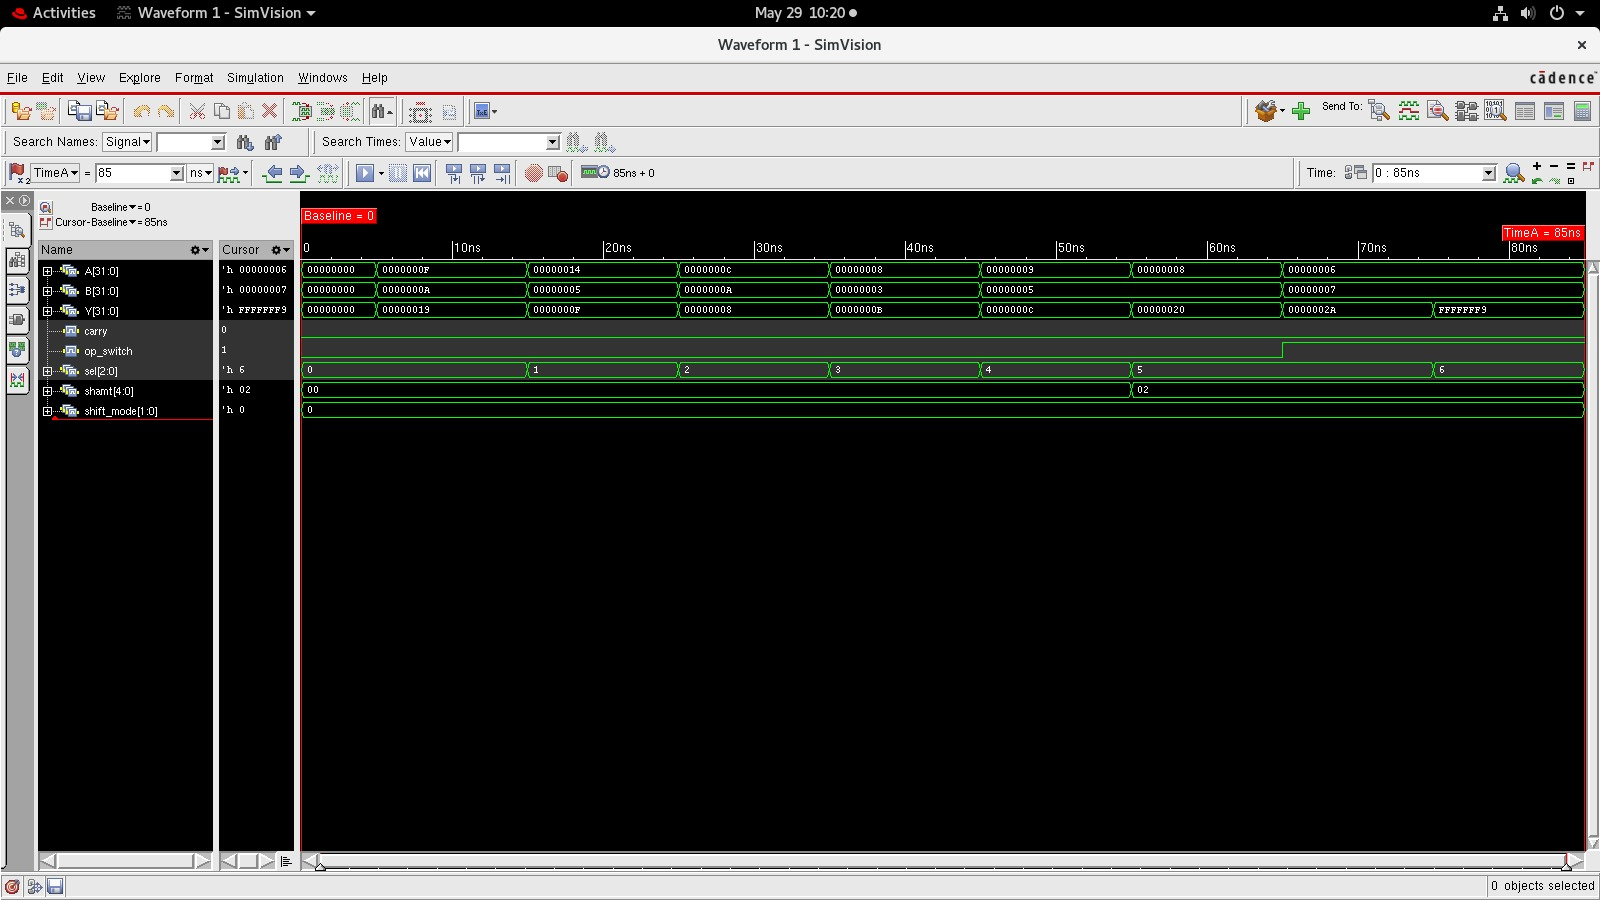
\includegraphics[width=8cm]{waveform.png}
\caption{Cadence Simulation Waveform}
\end{figure}
\section{Simulation and Waveform Analysis}

Functional verification and waveform analysis were performed using Cadence SimVision.

The simulation verified arithmetic, logical, shift, and multiplication operations successfully.Cadence SimVision wave forms analysis was used to check the functionality of the proposed ALU. The total duration of the simulation was 80ns and the duration for each operation was 10ns. The waveform shows the behaviour of the input signals, control signals and output responses for all the supported ALU operations. The outputs achieved are consistent with the outputs predicted, which is good evidence of the correct implementation of the design. The ALU executes ADD operation from 0 ns to 10 ns. The operands A and B are given the values of 7 and 12, respectively and the selection signal is set to addition. The output signal Y yields the value of 19, indicating that the arithmetic addition unit is working properly. The carry output is low because there is no overflow during the operation. The ALU performs the operation SUB on A = 20 and B = 5 in the time interval 10 ns less than 20 ns. The output Y changes to 15, as it should be given the subtraction performed. This verifies that subtraction is done correctly with the arithmetic operators in the ALU core. The AND operation is tested in between the times 20 ns and 30 ns, with values A = 12 and B = 10. The waveform indicates that the output value is 8, which is correct for a bitwise AND operation. This assures the correct processing of individual bits for both of the operands. Operands A = 8 and B = 3 are used to perform OR operation between them from 30 ns to 40 ns.At 30 ns to 40 ns, operands A = 8 and B = 3 are supplied to perform an OR operation between them. This prints out 11, as the bitwise OR operation was executed correctly. The output clearly demonstrates the change in values of the waveform as the input changes. The operation XOR is checked between 40ns and 50ns. When the inputs A = 9 and B = 5, the output is 12. The waveform validates the validity of the XOR operation by generating the correct output through a bitwise comparison of the two operands. The time range of 50 ns to 60 ns is related to the SHIFT operation. In this time the selection signal is active and the op\_switch is LOW, to choose the output of the Barrel Shifter. If the amount of shift, a, is 2, and the number of positions, A, is 8, the output is 32. The waveform shows that the Logical Shift Left operation is performed correctly in a single cycle, confirming the viability of the Barrel Shifter architecture. In the operation MULTIPLY is executed between 60 ns and 70 ns. The shared opcode is still alive, but op\_switch now is HIGH and allows the Booth Multiplier. When A = 6 and B = 7 the output should be 42. The waveform shows that it is working correctly to multiply and it's showing correct operation selection using the shared opcode mechanism. Lastly, the NOT operation is checked from 70 to 80 ns. Thus, the value of A is set to 8 and the output value FFFFFFF7 is the one's complement of A. The waveform verifies that all of the input bits are inverted bitwise and that the NOT is executed successfully. The waveform analysis results in the overall conclusion that the arithmetic, logical, shifting, multiplication and inversion operations are performed correctly. There are no functional errors in the transitions between operations and they are performed at the expected intervals. All eight test cases have been successfully verified, proving the reliability of the ALU architecture suggested in this work, and proving the correct interconnection of Booth Multiplier, Barrel Shifter, and the shared opcode control logic.

\begin{table}[h]
\renewcommand{\arraystretch}{1.3}
\setlength{\tabcolsep}{5pt}
\caption{Simulation Test Cases Results}
\label{tab:testcases}
\centering
\begin{tabular}{|c|c|c|c|c|}
\hline
\textbf{Time} & \textbf{Operation} & \textbf{Input} & \textbf{Output} & \textbf{Status} \\
\hline
0--10 ns & ADD & 7+12 & 19 & Verified \\
\hline
10--20 ns & SUB & 20--5 & 15 & Verified \\
\hline
20--30 ns & AND & 12 AND 10 & 8 & Verified \\
\hline
30--40 ns & OR & 8 OR 3 & 11 & Verified \\
\hline
40--50 ns & XOR & 9 XOR 5 & 12 & Verified \\
\hline
50--60 ns & SHIFT & $8 \ll 2$ & 32 & Verified \\
\hline
60--70 ns & MULTIPLY & $6 \times 7$ & 42 & Verified \\
\hline
70--80 ns & NOT & NOT 8 & FFFFFFF7 & Verified \\
\hline
\end{tabular}
\end{table}


\begin{table}[h]
\centering
\caption{Comparison of ALU Architectures}
\label{tab:final_comp}
\begin{tabular}{|l|c|c|c|c|}
\hline
\textbf{Parameter} & \textbf{Normal} & \textbf{+Booth} & \textbf{+Barrel} & \textbf{Proposed} \\
\hline
Operations Supported & 6 & 7 & 7 & 8 \\
\hline
Shift Delay (ns) & 2.84 & 2.85 & 0.65 & 0.66 \\
\hline
Multiply Delay (ns) & -- & 2.41 & -- & 2.42 \\
\hline
Area Increase (\%) & 0 & 28.9 & 75.8 & 83.5 \\
\hline
Power Increase (\%) & 0 & 39.8 & 122.7 & 158.1 \\
\hline
Shift Energy Reduction (\%) & -- & -- & 88 & 87 \\
\hline
Overall Capability & Low & Medium & Medium & High \\
\hline
\end{tabular}
\end{table}

Table~III presents a comparison of the four ALU architectures in terms of functionality, propagation delay, area, power consumption and energy efficiency. The conventional ALU consumes the least power and occupies the minimum space as it only supports 6 basic arithmetic and logical operations. It doesn't have dedicated multiplication hardware, nor high-speed shift operations, however. The Booth Multiplier based ALU adds functionality, with multiplication delay of 2.41~ns. Although the area and power increase by 28.9\% and 39.8\%, respectively, Booth multiplication reduces the number of partial products, resulting in faster multiplication. Likewise, the Barrel Shifter cuts the shift delay from 2.84~ns to 0.65~ns, which can achieve approximately 77\% faster shift operations by single cycle parallel shifting. The proposed ALU has been optimized with both optimizations and supports all the 8 arithmetic, logical, shift and multiplication operations. Multiplication can be done in 2.42~ns, shift can be done in 0.66~ns. The architecture expands by 83.5\%, the power consumption by 158.1\%, but the functionality and performance are greatly enhanced. A shared opcode mechanism with the shared control signal \texttt{op\_switch} reduces the complexity of the decoder and enhances the hardware resources utilization. All supported operations have been implemented correctly, verified and synthesized by functional verification and Cadence tools using Verilog HDL.The proposed architecture also lowers the shift energy to 3.12~pJ which is about 87\% lower than 23.14~pJ. The results show that the proposed Booth Multiplier and Barrel Shifter integrated ALU is able to provide a good hardware cost, computational speed and energy efficiency which can be used in modern processors and embedded applications.

\section{Conclusion}

This paper presents the design, verification, and synthesis of an optimized 32-bit ALU using a Booth Multiplier and a Barrel Shifter. The architecture was built and tested for the synthesis of application-specific integrated circuits (ASICs) and is capable of performing 8 types of arithmetic, logic, shift, and multiplication operations. It uses the shared opcode approach for the control unit, which has allowed decreasing both the complexity of the opcode decoding process and the number of required opcodes. Verification of the design showed that the ALU correctly performs all operations. In addition, the number of transistors and power consumption of the synthesized design were found to be acceptable.

The Booth Multiplier and Barrel Shifter utilization have allowed for optimizing the architecture and achieving faster computations due to their ability to reduce the number of partial products during multiplication and perform all types of shifts within a single clock cycle, respectively. The shared opcode approach used in this design also contributed to the overall effectiveness of the ALU as it allowed to minimize the number of transistors needed for its implementation and thus reduced the complexity of the opcode decoding process.

Thus, the proposed ALU design is suitable for implementation in ASICs for embedded processors, digital signal processors, field-programmable gate arrays, and other systems requiring a high-performance arithmetic-logic unit. Future research will be aimed at developing an improved ALU with extended sets of arithmetic operations and advanced power-saving capabilities.



\begin{thebibliography}{15}

\bibitem{ref1}
V. V. N. Phanindrakumar, P. K. Hota, and V. Kamakoti, ``32-Bit ALU Using Different Adders,'' \emph{International Conference}, 2018.

\bibitem{ref2}
Rakshith C., S. Chethan, M. Charan, and M. S. Rekha, ``Design and Implementation of High Speed ALU Using 32-Bit Barrel Shifter,'' \emph{International Journal of Engineering Research and Technology}, 2022.

\bibitem{ref3}
J. S. D. Vudatha, N. Kota, P. Gutha, B. Sreeja, and S. P. Rajeev, ``VLSI Design of Low Power 8×4 Barrel Shifter Using 90 nm Transmission Gate Technology,'' in \emph{Proc. IEEE Conference}, 2021.

\bibitem{ref4}
W. C. Yeh, C. W. Jen, and Y. T. Hwang, ``High-Speed Booth Encoded Parallel Multiplier Design,'' \emph{IEEE Transactions on Computers}, vol. 49, no. 7, pp. 692--701, 2000.

\bibitem{ref5}
N. Pandey and S. Gupta, ``Design and Implementation of Novel Multiplier Using Barrel Shifters,'' \emph{International Journal of Image, Graphics and Signal Processing}, vol. 7, no. 8, pp. 28--34, 2015. 

\bibitem{ref6}
M. G., A. L. Kulkarni, and J. S. Baligar, ``ASIC Implementation of High Speed and Low Power ALU,'' \emph{International Journal of Engineering Research \& Technology (IJERT)}, vol. 8, no. 7, 2019. 

\bibitem{ref7}
M. Kathirvelu and T. Manigandan, ``Design and Implementation of High Speed ALU Using Optimized PDP Adder and Multiplier,'' \emph{Journal of Applied Sciences Research}, vol. 8, no. 4, pp. 2100--2108, 2012. 

\bibitem{ref8}
R. Choubey and M. Arif, ``Area Optimized and Low Power Using Modified Booth Multiplier for Unsigned Numbers,'' \emph{International Journal of Emerging Science and Engineering}, vol. 2, no. 6, pp. 28--32, 2014. 

\bibitem{ref9}
L. Khan, ``Designing Low Power High Speed 32-Bit Barrel Shifter for ARM7 Processor,'' \emph{International Journal of Advanced Research in Computer Science}, vol. 4, no. 3, pp. 108--111, 2013.

\bibitem{ref10}
M. Waghela, S. Kumari, and S. Kumari, ``VLSI Design of Low Power Barrel Shifter Using Pseudo Dynamic Logic,'' \emph{International Journal of Science, Engineering and Technology}, vol. 2, no. 6, pp. 750--757, 2014. 

\bibitem{ref11}
Z. Chaithanya and U. Penchalaiah, ``Design and Simulation of Low-Power VLSI Multiplier Using Modified Booth Algorithm,'' \emph{International Journal of Emerging Research in Science, Engineering and Management}, vol. 1, no. 4, pp. 27--32, 2025.

\bibitem{ref12}
P. Sandeep, A. Ugadi, P. Rajkumar, P. PavanKalyan, and D. Vikranth, ``32-Bit Arithmetic Logic Unit Development Using Verilog HDL: Design and Implementation,'' \emph{International Journal of Creative Research Thoughts}, vol. 13, no. 5, 2025. 

\bibitem{ref13}
C. S. Wallace, ``A Suggestion for a Fast Multiplier,'' \emph{IEEE Transactions on Electronic Computers}, vol. EC-13, no. 1, pp. 14--17, 1964.

\bibitem{ref14}
R. P. Brent and H. T. Kung, ``A Regular Layout for Parallel Adders,'' \emph{IEEE Transactions on Computers}, vol. C-31, no. 3, pp. 260--264, 1982.

\bibitem{ref15}
D. A. Patterson and J. L. Hennessy, \emph{Computer Organization and Design: The Hardware/Software Interface}, 5th ed. Morgan Kaufmann, 2014.

\end{thebibliography}



\end{document}